% !TEX root = catron-dissertation.tex
\epstopdfsetup{outdir=./images/08_conclusion/}

\chapter{Conclusion}
\label{chap:08_conclusion}
% \textcolor{red}{
%   \begin{itemize}
%     \item
%   \end{itemize}
% }

When aero-optical measurements are made in a wind tunnel, there are a number of sources that contaminate the measurement with noise.
This can be seen in Figure \ref{fig:08_dispersion_isosurface} which shows a multidimensional spectral estimation of an optical wavefront measurement made in a wind tunnel.
\begin{figure}
  \centering
  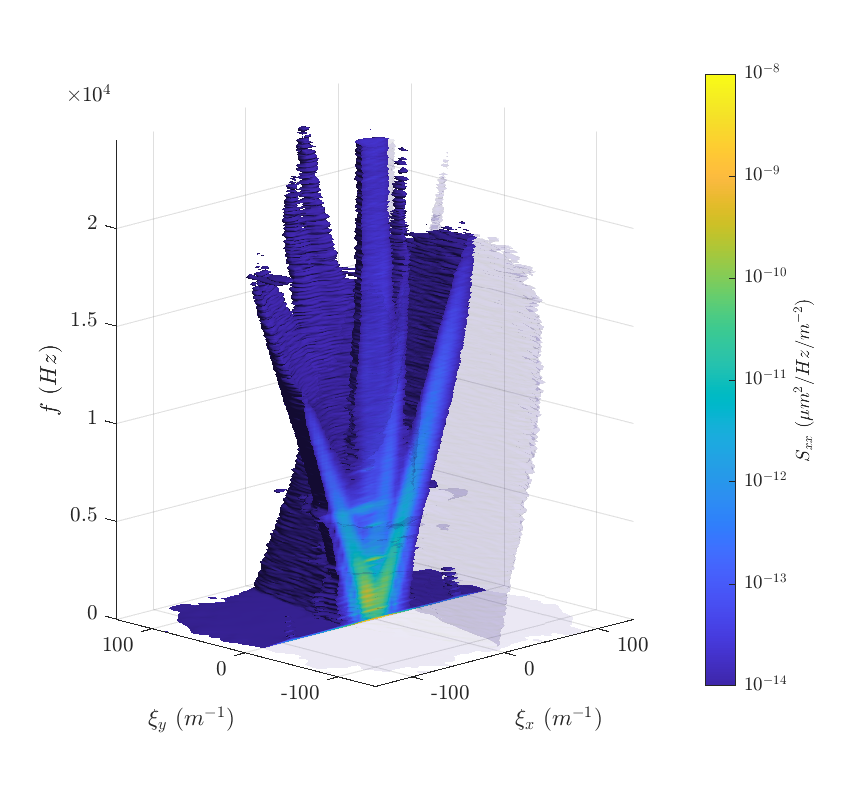
\includegraphics{../matlab/08_conclusion/dispersion_isosurface.eps}
  \put(-195,120){\rotatebox{76}{\Large Boundary Layer}}
  \put(-305,250){\rotatebox{-75}{\Large Acoustic Cone}}
  \put(-300,69){\textcolor{white}{\Large BPF $\Longrightarrow$}}
  \put(-231,180){\textcolor{white}{\rotatebox{90}{\Large Stationary Modes}}}
  \put(-235,50){\rotatebox{15}{\Large Mean-Lensing}}
  \caption{Multidimensional spectral estimation of an optical wavefront measurement made in a wind tunnel.}
  \label{fig:08_dispersion_isosurface}
\end{figure}
Figure \ref{fig:08_dispersion_isosurface} shows the full multi-dimensional spectrum for wavefront data acquired in a wind tunnel, including streamwise and vertical spatial frequencies ($\xi_x$ and $\xi_y$), and temporal frequencies ($f$); however, in
in Figure \ref{fig:08_dispersion_isosurface}, the half of the isosurface which represents the portion of the signal that has a component that is traveling vertically downward has been made transparent to show some of the internal power spectrum of planar waves that are traveling parallel to the direction of flow.

In Figure \ref{fig:08_dispersion_isosurface}, the aero-optical signal that is considered to be the objective of the measurement is the boundary layer which resembles a thin ellipsoid that has an angle in the $x-\xi_x$ plane (where the $xi_x$-coordinate represents spatial frequencies in the stream-wise direction) by an amount related to the free-stream velocity (see Equation \ref{eqn:04_velocity_assumed}).
Acoustic duct modes make up a temporally broadband signal that forms a cone and have a significant portion of the signal that travels upstream.
In the $\xi_x-f$ plane the outer surface of the acoustic cone is limited by the sonic lines at $u\pm c$, while in the $\xi_y-f$ plane the limit is at $\pm c$.
The wind-tunnel fan produces temporally narrow-band acoustic and vibration modes that are able to contaminate the wavefront measurement at the blade-passing frequency (BPF) and its various harmonics.

Sources of noise shown in Figure \ref{fig:08_dispersion_isosurface} not related to the acoustics include stationary modes and mean-lensing.
The stationary modes do not travel in any direction, their spatial frequencies are near zero and their signal strength is fairly constant in time.
Due to the temporally white-noise nature of this signal, it is likely not physically relevant and could be optical mode noise from the laser, electronic noise in the camera, or even numerical noise from the processing code.
At lower frequencies, especially around the blade-passing frequency or its harmonics, there is likely a significant number of stationary modes that are due to vibration of various optical elements.
The mean-lensing portion of the signal ($\lessapprox 100$ Hz) is a slowly varying signal with large spatial frequency content.
A color coded multidimensional spectral estimation plot that allows for easier identification of the various component signals is shown in Figure \ref{fig:05_synthetic_dispersion_input} and was used for generating a synthetic wavefront.
As such, a major contribution of this dissertation research is an improved understanding of the signals and contamination that appear in aero-optical data, and how those signals appear in multi-dimensional spectra. This information provides a better understanding of aero-optical data, as well as guidance towards methods of filtering out contaminating noise sources.

\section{Filtering of Optical Wavefronts}
Two main families of filtering techniques were examined in this dissertation.
The first family was single sensor filters, Chapter \ref{chap:06_single_filter}, which operate on the optical wavefronts without knowledge of any other time resolved data.
Some of these filters may rely on additional information about the average sampling conditions used to measure the wavefronts.
The second family was multiple sensor filters, Chapter \ref{chap:07_multiple_filter}, which filter the optical wavefront using time resolved measurements from additional sensors.

\subsection{Single Sensor Filters}
The single sensors filters operated directly on the optical wavefront measurements.
Most of these filters are based on Butterworth filters \cite{Butterworth-1930-DvDrjKha} that operate in the multidimensional Fourier domain using a transfer function, $\hat{H}(\xi_x,\xi_y,f)$,
\begin{equation}
  \widehat{WF}(\xi_x,\xi_y,f) = \hat{H}(\xi_x,\xi_y,f)\fftthree(wf(x,y,t)) \textrm{,}
\end{equation}
which can be inverse Fourier transformed back into the physical domain or be used for calculating the multidimensional spectrum.
Filtering can also be performed on the multidimensional spectrum using the gain function, $G^2 = \hat{H}\hat{H}^*$,
\begin{equation}
  S_{xx}(\xi_x,\xi_y,f) = G^2(\xi_x,\xi_y,f)S_{xx}(\xi_x,\xi_y,f) \textrm{.}
\end{equation}
The only filter that was investigated that was not based on basic filters was a baseline spectrum estimator \cite{Schulze-2012-GmyAqzC7}.
This filter removes narrow-band peaks and noise peaks along the temporal frequency axis smooth spectrum.

\section{Other Useful Products}

\subsection{Synthetic Wavefront}
A synthetic wavefront was developed in Chapter \ref{chap:05_synthetic} to test various filters used in Chapter \ref{chap:06_single_filter}.
In the process used to create the synthetic wavefront, each of these signal components was generated separately in the multidimensional spectrum.
While this synthetic wavefront generation technique produced a qualitative approximation of a wavefront, it provided a useful set of fully known data to test various filters.
There is some significant room for improvement in the process of creating synthetic wavefronts that are more physically accurate.
Even without improvement this process may be useful in generating a set of synthetic wavefronts with a known aero-optical and noise components that can be used for training a neural network to filter \cite{Lo-1994-W6aWeuaT} wavefront measurements.
A neural network based filter may be able to separate the overlapping component signals at low frequencies.

\subsection{Measuring Acoustic Field Optically}
In section \ref{sect:03_examples_spherical}, optical wavefront were shown to have a fairly good agreement with a microphone for measuring the fluctuating field strength of a spherical wave generated by a speaker.
The optical wavefront measurement however had issues when the acoustic field diverged from being nearly spherical.
Optical wavefronts can be a method to non-intrusively measure an acoustic field, although the beam-path integrated results of the wavefront measurement require additional interpretation to extract information on the acoustic field.

\subsection{Acoustic Mode-Marching}
An acoustic mode-marching method was developed to quickly estimate the acoustic field within a wind-tunnel test-section assuming that the primary noise source was the wind-tunnel fan.
Although, this is likely to have limited application in filtering of optical wavefronts, it is useful for assisting researchers in determining whether specific narrow-band signals are produced by the wind-tunnel fan and can be filtered out.
Since there may be upstream-traveling components of the aero-optical signal such as that produced by recirculation zones or sound produced by the test model, the capability to definitively identify the optical signal produced by the wind-tunnel main fan is useful information.
There also maybe some application during the initial design of a tunnel for estimating the acoustic field in some critical components.

\section{Recommendations For Future Research}

Future research is needed to better validate these filtering techniques as well as aid in the development of future filtering techniques.
This in part can be accomplished by making a series of measurements on different models that differ only in scale.
For turrets the aero-optical signal can be normalized \cite{Jumper-2013-8KtN3pue},
\begin{equation}
  \opd_{NORM} = \frac{\opd}{\left(\frac{\rho_0}{\rho_{SL}}\right)M^2D} \textrm{,}
\end{equation}
where $\rho_0$ is the free-stream total density of the flow around the turret, $\rho_{SL}$ is the density of air at sea-level, and $D$ is the turret diameter.
This equation allow the aero-optical signal to be scaled to different models.
Test results from different scale models should be in agreement after the signal contamination is removed.

A detailed set of measurements should be produced capturing not only the aero-optical mesurements but also simultaneous sound and vibration measurements.
This has been partially done before with hemispherical and hemisphere-on-cylinder turrets, but other geometries such as partial-hemisphere or generic-pod-based geometries need a test database as well.
Optical wave-front measurements behind a turbulent wake from a cylinder may even prove to be useful.

There is a lot of research that can still be done on various filtering techniques to remove signal contamination of aero-optical wavefront measurements.
This is especially true for filters that can utilize additional sensor measurements.
The process for creating the synthetic wavefronts used in this research was a qualitative approximation that can be made more physically accurate.
Synthetic signal algorithms could be developed for types other aero-optical disturbances such as sheer layers \cite{Jumper-2017-8UnkaeqW}.
Synthetic wavefront signals could aid in the testing of algorithms used on adaptive optic systems.
The acoustic mode-marching analysis could be expanded to the case where a simple model in the wind-tunnel test section.
